\section{クラスタリング実験}

\subsection{実験環境}
実験にはPython3.5を用い,
機械学習のライブラリとしてTensorFlowを用いてアルゴリズムを実装した.

\subsection{精度の評価}
クラスタリング精度の評価はPythonのライブラリであるscilit-learnを用い,以下の3項目により行った.
\begin{description}
  \item[ARI; Adjusted Rand Index, 調整ランド指数]~\\
    クラスタの正解ラベルに対してクラスタリング結果の一致度を評価する指標.1に近づくほどよい結果.
  \item[NMI; Normalized Mutual Information, 正規化相互情報量]~\\
    相互情報量を正規化した尺度.
  \item[Purity]~\\
    生成されたクラスタがどれだけ多数派で占められているかを表す尺度
\end{description}

また,推定されたクラスタ数および,複数回クラスタリングを繰り返し,その際に推定されたクラスタ数の分散も算出した.

\subsection{2次元空間のクラスタリング}

まず,2次元のデータのクラスタリング結果を比較する.
2次元空間に分散$\sigma^2=1$のGauss分布により生成した,クラスタあたりのサンプル数を500として5つのクラスタを生成し,
対数尤度関数,BIC, AIC, cAICを分割停止規準として採用してクラスタリングを行った.

\tablenum{table:2dim}に都度ランダムに生成されたデータに対して100回クラスタリングを行ったときの,
推定されたクラスタ数,ARI, NMI, Purityの平均値および推定されたクラスタ数の分散を示す.
また,\figurenum{fig:2dim}に2次元空間におけるクラスタリングの例を示す.

\begin{table}[htb]
  \centering
  \caption{2次元空間におけるクラスタリング結果}
  \label{table:2dim}
  \begin{tabular}{|c|c|c|c|c|} \hline
    分割停止規準 & クラスタ数(分散) & ARI & NMI & Purity \\\hline
    BIC & 4.58 (0.9836) & 0.84458792 & 0.88281495 & 0.84458792\\
    cAIC & 4.55 (0.6475) & 0.85329139 & 0.89992544 & 0.85329139\\
    AIC & 4.69 (3.8739) & 0.83642236 & 0.88147442 & 0.83642236\\
    対数尤度関数 & 5.32 (10.236) & 0.85699618 & 0.91572100 & 0.85699618\\\hline 
  \end{tabular}
\end{table}

\tablenum{table:2dim}より,2次元空間においてXmeansの分割停止規準としてBICとcBICの間には
クラスタリング結果に大きな差がないことが読み取れる.
クラスタ数の推定もおおよそ適当であり,推定したクラスタ数の分散もあまり大きな値とはなっていない.

また,AICを分割停止規準として採用した場合に着目すると,推定したクラスタ数の分散が非常に大きくなっている.
これは,3.3節で述べたように,AICはパラメータ数を過大に見積もってしまうことに起因するものと思われる.
実際に,推定されたクラスタ数を見ると,クラスタ数を20や22と推定しているものが多く存在する.
しかし,素の対数尤度関数を分割停止規準として採用した場合のクラスタリング結果と比較すると,
比較的安定したクラスタ数推定を行っていることが見て取れる.

\begin{figure}[htbp]
  \begin{center}
    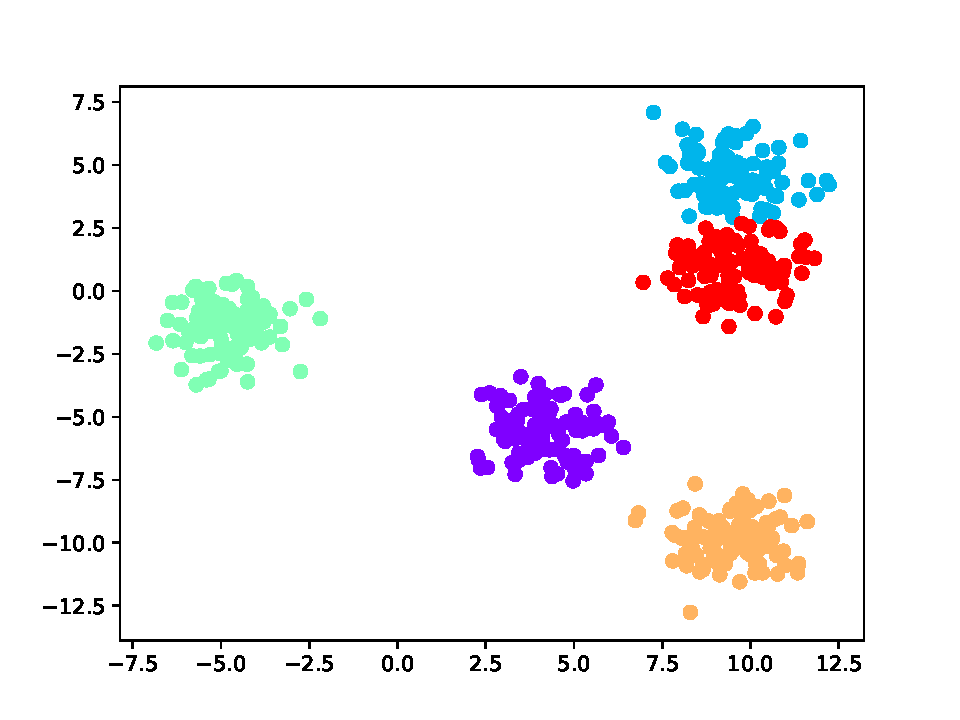
\includegraphics[width=0.7\linewidth]{./img/BIC_2.pdf}
      \caption{2次元空間のクラスタリング例}
      \label{fig:2dim}
  \end{center}
\end{figure}

\subsection{3次元空間のクラスタリング}

3次元空間に分散$\sigma^2=1$のGauss分布により生成した,クラスタあたりのサンプル数を500として5つのクラスタを生成し,
対数尤度関数,BIC, AIC, cAICによりクラスタリングを行った.

\tablenum{table:3dim}に都度ランダムに生成されたデータに対して100回クラスタリングを行ったときの,
推定されたクラスタ数,ARI, NMI, Purityの平均値および推定されたクラスタ数の分散を示す.

また,\figurenum{fig:3dim}に2次元空間におけるクラスタリングの例を示す.

\begin{table}[htb]
  \centering
  \caption{3次元空間におけるクラスタリング結果}
  \label{table:3dim}
  \begin{tabular}{|c|c|c|c|c|} \hline
    分割停止規準 & クラスタ数(分散) & ARI & NMI & Purity \\\hline
    BIC & 4.95 (0.0669) & 0.97179074 & 0.97913818 & 0.97179074\\
    cAIC & 4.92 (0.2313) & 0.96312702 & 0.97023920 & 0.96312702\\
    AIC & 4.88 (0.1443) & 0.95216819 & 0.96855698 & 0.95216819\\
    対数尤度関数 & 5.12 (4.1443) & 0.95731637 & 0.96541468 & 0.95731637\\\hline 
  \end{tabular}
\end{table}

\begin{figure}[htbp]
  \begin{center}
    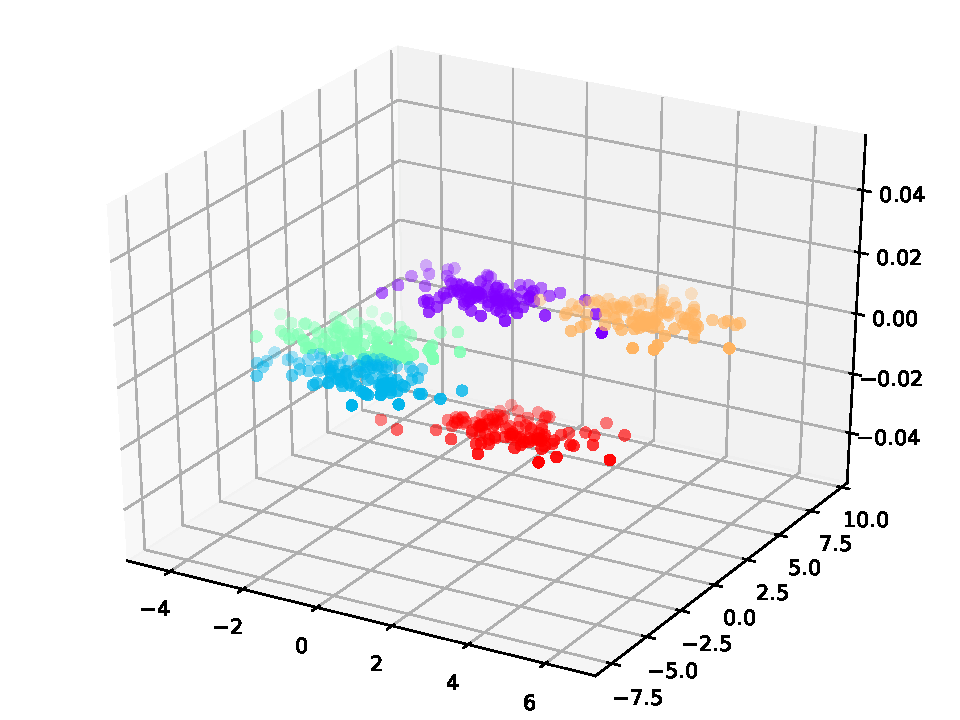
\includegraphics[width=0.7\linewidth]{./img/BIC_3.pdf}
      \caption{3次元空間のクラスタリング例}
      \label{fig:3dim}
  \end{center}
\end{figure}
2次元のクラスタリングとは異なり,3次元空間においてはBICを分割停止規準として採用した場合の精度が良くなっている.
分散値も非常に小さいため,安定して精度の高いクラスタリングを行っていることが伺える.

cAICとAICの場合を比較した場合,cAICのほうがクラスタリングの精度が高いことがわかる.
しかし,AICにおけるクラスタリングでは,2次元空間ほど推定されたクラスタ数の分散が大きくないことがわかる.
2次元空間では,クラスタ数を過大に見積もってしまう問題があったが,
3次元空間においてその問題は発生していなかった.

